\chapter{测试报告}

\section{测试策略}

测试目标是证明重构没有破坏核心外部行为，并且本地提交版本具备可复现的运行、构建和验收流程。本次测试分为三层：

\begin{itemize}
  \item 工程基线测试：确认前端 lint、生产构建和后端 pytest 可以稳定执行。
  \item 接口烟测：确认登录、系统时间、预测模型列表、预测参数和 future 数据接口可用。
  \item 浏览器验收：确认管理员登录后可以访问仪表盘、站点管理、调度管理、需求管理和设置页面。
\end{itemize}

原始命令输出保存在 \code{docs/refactoring_report_tex/evidence/}，截图证据保存在 \code{docs/refactoring_report_tex/figures/evidence/}。

\section{测试环境}

\begin{longtable}{p{0.25\textwidth}p{0.55\textwidth}}
\toprule
项目 & 配置 \\
\midrule
前端地址 & \code{http://127.0.0.1:5173/} \\
后端地址 & \code{http://127.0.0.1:5000/} \\
MySQL & \code{127.0.0.1:3307} \\
管理员账号 & \code{admin/admin123} \\
调度员账号 & \code{dispatcher/dispatcher123} \\
运维账号 & \code{operator/operator123} \\
\bottomrule
\end{longtable}

\section{自动化测试}

\begin{longtable}{p{0.26\textwidth}p{0.36\textwidth}p{0.25\textwidth}}
\toprule
测试项 & 命令 & 结果 \\
\midrule
前端 Lint & \code{npm run lint} & 通过，0 errors，保留 warnings \\
前端构建 & \code{npm run build} & 通过，存在大 chunk 警告 \\
后端测试 & \code{python -m pytest} & 20 passed, 4 skipped \\
\bottomrule
\end{longtable}

后端新增的重构工具测试覆盖统一响应、错误装饰器、角色装饰器、路径配置和预测模型注册表。前端 lint 当前已经没有阻塞 error，剩余 warning 主要来自历史模板页面、\code{any} 类型和部分 hook 依赖提示，记录为后续低风险清理项。

\section{接口烟测}

系统时间接口：

\begin{quote}
\code{GET http://127.0.0.1:5000/api/system/time}
\end{quote}

返回示例：

\begin{verbatim}
{
  "current_time": "2026-06-15T14:50:11",
  "mode": "real",
  "timezone": "Asia/Shanghai"
}
\end{verbatim}

登录接口使用 \code{admin/admin123} 可以返回 access token，前端可进入受保护页面。

\begin{figure}[H]
  \centering
  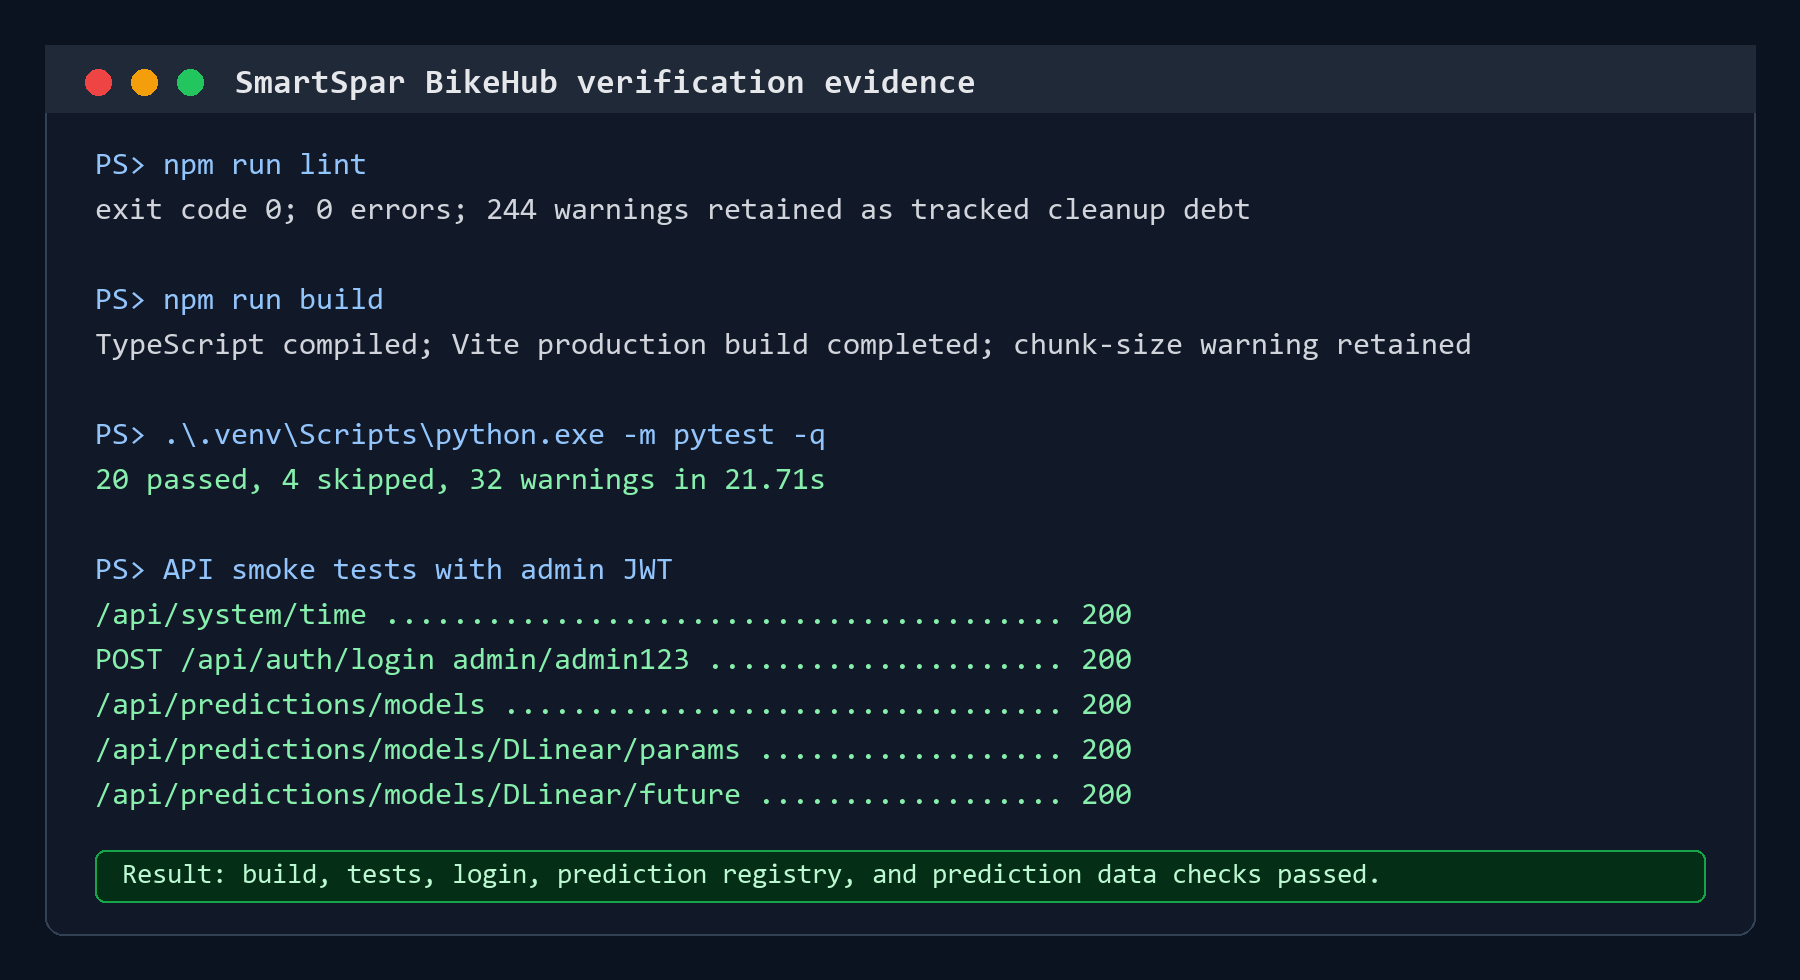
\includegraphics[width=0.92\textwidth]{figures/evidence/terminal_verification.png}
  \caption{命令行验证结果摘要}
\end{figure}

预测相关接口烟测结果如下：

\begin{longtable}{p{0.55\textwidth}p{0.15\textwidth}p{0.2\textwidth}}
\toprule
接口 & 状态 & 验证目的 \\
\midrule
\code{/api/predictions/models} & 200 & 模型注册表可读 \\
\code{/api/predictions/models/DLinear/params} & 200 & 参数文件可读 \\
\code{/api/predictions/models/DLinear/future} & 200 & future 分页数据可读 \\
\bottomrule
\end{longtable}

\section{浏览器与预测验收}

\begin{longtable}{p{0.28\textwidth}p{0.5\textwidth}p{0.12\textwidth}}
\toprule
验收项 & 验收结果 & 状态 \\
\midrule
登录页 & 管理员账号 \code{admin/admin123} 可登录，登录后进入受保护页面 & 通过 \\
仪表盘 & 展示运营总览、任务统计、系统时间、地图区域和站点排行 & 通过 \\
站点管理 & 展示演示站点，搜索、列视图和表格布局可用 & 通过 \\
调度管理 & 展示演示调度任务，状态和操作入口可见 & 通过 \\
需求管理 & 实时需求记录可见，旧路径 \code{/demand_management} 自动跳转 & 通过 \\
设置页面 & 外观、侧栏、布局和阅读方向配置已融入正式设置页 & 通过 \\
预测功能 & \code{DLinear}、\code{TiDE}、\code{TimesNet} 标签可见，DLinear future 数据可渲染 & 通过 \\
\bottomrule
\end{longtable}

\section{遗留风险与后续处理}

\begin{longtable}{p{0.36\textwidth}p{0.42\textwidth}p{0.12\textwidth}}
\toprule
风险项 & 后续处理建议 & 影响 \\
\midrule
前端 lint 仍有 warning & 按模块清理历史模板残留、\code{any} 类型、未使用 import、console 和 hook 依赖提示 & 低 \\
Vite 提示部分 chunk 大于 500 KB & 通过路由懒加载和 manual chunks 优化首屏资源 & 低 \\
SQLAlchemy relationship overlap warning & 通过 \code{back_populates}、\code{viewonly} 或 \code{overlaps} 修正模型关系 & 中 \\
重新训练预测模型需要 torch 环境 & 将训练环境与演示运行环境分离，提交说明中保留可选安装步骤 & 中 \\
\bottomrule
\end{longtable}
